\clearpage
\subsection{Usability testing}
Usability testing is a test in which whether a user achieves the intended functional goal using a system or not, and the level of effort involved to use the system and achieve the intended functional goal.\cite{iso:9126}. The success of a usability test is dependent on the goal of the usability test. A usability test should have a specified goal, a carefully prepared questionnaires, appropriate techniques and tools to be of any use. The most frequently used method of conducting a usability test is based on four notable points\cite{usability:doc2}\cite{usability:doc3}.

%\begin{itemize}
%\item Efficiency - time to complete task
%\item Effectiveness - task completed ratio
%\item Learnability - number of errors recorded for novice users
%\item Memorability - browsing and searching for non-regular users
%\end{itemize}

Another method of measuring user attitude towards a system is TAM.
TAM, technology acceptance model, is a tool with which users general perceived of use, perceived ease of use and intention to use is measured. While usability testing is more focused on  task based performance of users\cite{tam:doc4}, TAM is a general attitude test based on a twelve question model in which 3 things are measured

\begin{itemize}
\item PU - Perceived usefulness, how the user considers the system useful
\item PEU - Perceived ease of use, how the user considers the system easy to use
\item ITU - Intention to use, how likely is the user to want to use the system again
\end{itemize}

\begin{figure}[htb]
	\centering
	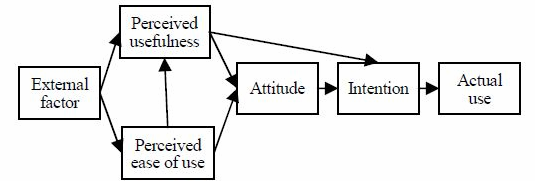
\includegraphics[width=0.8\textwidth]{reqspec/tam.png}
	\caption{Technology acceptance model framework\cite{tam:doc4}}
	\label{fig:tam}
\end{figure}

In this project, we will be using a revised version of the usability test we described above, especially focusing on effectiveness and efficiency. Artsdatabanken has an already web experienced user base and the number of novice users might probably not be significant to measure memorability and learnability of the system.
To measure performance and perception with regard to the system, the team will use a post questionnaire in the form of the three TAM categories. Learnability will also be explored using TAM.

\begin{table}[h]
\centering
\caption{Use case scenario usability testing\cite{tam:doc5}} % title of Table

\begin{tabular}{|c|c|c|c|c|c|p{3cm}|} % centered columns (6 columns)
\hline\hline %inserts double horizontal lines
Use case ID & Description & Pre conditions & Post conditions & Time spent & error count \\

\hline % inserts single horizontal line
F1 & Create new  & User wants to  & A new observation  & 10min & 2 \\
\hline
F2 & - & - & - & - & - \\
F3 & - & - & - & - & -\\
F5 & - & - & - & - & -\\
\hline %inserts single line
\end{tabular}
\label{table:nonlin} % is used to refer this table in the text
\end{table}

%Perception test using a TAM Post questionnaire\cite{tam:doc4}\cite{tam:doc6}

